\documentclass[a4paper]{article}

\def\nbook {All of Statistics: A Concise Course in Statistical Inference}
\def\nbookshort {All of Statistics}

% Shared preamble. The fallback lets the document build whether the working
% directory is its own folder or the project root.
\IfFileExists{header.tex}{\input{header}}{%%%%%%%%%%%%%%%%%%%%
% AUTHOR AND HEADER
% define \nbook
%%%%%%%%%%%%%%%%%%%%

\makeatletter
\ifx \nauthor\undefined
  \def\nauthor{David A. Lee}
\else
\fi

\author{\nbook \\ \small Solutions by \nauthor}
\date{}

%%%%%%%%%%%%%%%%%%%%
% PACKAGES
%%%%%%%%%%%%%%%%%%%%

\usepackage{alltt} 
\usepackage{amsfonts}
\usepackage{amsmath}
\usepackage{amssymb}
\usepackage{amsthm}
\usepackage{bm}
\usepackage{booktabs}
\usepackage{caption}
\usepackage{centernot}
\usepackage{enumitem}
\usepackage{fancyhdr}
\usepackage[T1]{fontenc}
\usepackage{graphicx}
% Images live in chap1/ ... chap8/ at the project root, while the documents that
% use them sit one level down (allofstats/, allofstatschap1/, ...). Listing both
% "./" and "../" lets a document keep writing \includegraphics{chap1/foo.eps}
% and still resolve it whether it is compiled from its own folder or from the
% project root.
\graphicspath{{./}{../}}
\usepackage{mathdots}
\usepackage{mathtools}
\usepackage{microtype}
\usepackage{multirow}
\usepackage{pdflscape}
\usepackage{pgfplots}
\pgfplotsset{compat=1.18}
\usepackage{siunitx}
\usepackage{slashed}
\usepackage{tabularx}
\usepackage{tikz}
\usepackage{titletoc}
\usepackage{tkz-euclide}
\usepackage[normalem]{ulem}
\usepackage{url}
\usepackage[all]{xy}
\usepackage{imakeidx}

% fonts
% use \textsf to change to Computer Modern Bright
\renewcommand{\sfdefault}{cmbr} % keeps default font Computer Modern Roman

% makeindex for table of contents
\makeindex[intoc, title=Index]
\indexsetup{othercode={\lhead{ Index }}}

% table of contents remove numbering
\setcounter{secnumdepth}{0}

% pagestyle
\pagestyle{fancyplain}

% header
\lhead{	\nouppercase{\leftmark} }
\ifx \nextra \undefined
  \rhead{
    \ifnum\thepage=1
    \else
      \nbookshort \  | \nauthor
    \fi}
\else
  \rhead{
    \ifnum\thepage=1
    \else
      \nbookshort (\nextra)
    \fi}
\fi

% proof environment

\newcommand{\prooffont}{\scshape}
\usepackage{xpatch}
\tracingpatches
\xpatchcmd{\proof}{\itshape}{\prooffont}{}{}

% Python environment (for typesetting Python code)

% Default fixed font does not support bold face
\DeclareFixedFont{\ttb}{T1}{txtt}{bx}{n}{8} % for bold
\DeclareFixedFont{\ttm}{T1}{txtt}{m}{n}{8}  % for normal

% Custom colors
\usepackage{color}
\definecolor{deepblue}{rgb}{0,0,0.5}
\definecolor{deepred}{rgb}{0.6,0,0}
\definecolor{deepgreen}{rgb}{0,0.5,0}

\usepackage{listings}

% Python style for highlighting
\newcommand\pythonstyle{\lstset{
language=Python,
basicstyle=\ttm,
morekeywords={self},              % Add keywords here
keywordstyle=\ttb\color{deepblue},
emph={MyClass,__init__},          % Custom highlighting
emphstyle=\ttb\color{deepred},    % Custom highlighting style
stringstyle=\color{deepgreen},
frame=tb,                         % Any extra options here
showstringspaces=false
}}


% Python environment
\lstnewenvironment{python}[1][]
{
\pythonstyle
\lstset{#1}
}
{}

% Python for external files
\newcommand\pythonexternal[2][]{{
\pythonstyle
\lstinputlisting[#1]{#2}}}

% Python for inline
\newcommand\pythoninline[1]{{\pythonstyle\lstinline!#1!}}

%%%%%%%%%%%%%
% FUNCTIONS %
%%%%%%%%%%%%%

\DeclarePairedDelimiter\abs{\lvert}{\rvert}%
\DeclarePairedDelimiter\norm{\lVert}{\rVert}%

%%%%%%%%%%%%%%%%%%%%
% DOCUMENT GEOMETRY
%%%%%%%%%%%%%%%%%%%%

\ifx \ntrim \undefined
\else
  \usepackage{geometry}
  \geometry{
	  papersize={379pt, 699pt},
	  textwidth=345pt,
	  left=17pt,
	  top=54pt,
	  right=17pt,
  }
\fi

% maketitle statement
\title{}
\ifx \nisofficial \undefined
\let\@real@maketitle\maketitle
\renewcommand{\maketitle}{\@real@maketitle\begin{center}\begin{minipage}[c]{0.9\textwidth}\centering\footnotesize All errors, typographical and substantive, and other offenses, are entirely my own.\end{minipage}\end{center}}
\else
\fi

%%%%%%%%%%%%%%%%%%%%
% THEOREMS
%%%%%%%%%%%%%%%%%%%%

%\theoremstyle{definition}
\newtheorem*{axiom}{Axiom}
\newtheorem*{claim}{Claim}
\newtheorem*{conjecture}{Conjecture}
\newtheorem*{cor}{Corollary}
%\newtheorem*{dfn}{Definition}
\newtheorem*{eg}{Example}
\newtheorem*{ex}{Exercise}
%\newtheorem*{lemma}{Lemma}
\newtheorem*{prop}{Proposition}
%\newtheorem*{thm}{Theorem}
\newtheorem*{remark}{Remark}
\newtheorem*{warning}{Warning}

%%%%%%%%%%%%%%%%%%%%
% FORMATTING AESTHETICS
%%%%%%%%%%%%%%%%%%%%

% itemize bullets
\renewcommand{\labelitemi}{-}
\renewcommand{\labelitemii}{$\circ$}
\renewcommand{\labelenumi}{(\roman{*})}

% new page section
\let\stdsection\section
\renewcommand\section{\newpage\stdsection}

%%%%%%%%%%%%%%%%%%%%
% \mathbb commands
%%%%%%%%%%%%%%%%%%%%

\newcommand{\C}{\mathbb{C}}
\newcommand{\N}{\mathbb{N}}
\newcommand{\Q}{\mathbb{Q}}
\newcommand{\R}{\mathbb{R}}
\newcommand{\Z}{\mathbb{Z}}


%%%%%%%%%%%%%%%%%%%%
% Probability Operators
%%%%%%%%%%%%%%%%%%%%

\DeclareMathOperator{\Bernoulli}{Bernoulli}
\DeclareMathOperator{\betaD}{Beta}
\DeclareMathOperator{\bias}{\textsf{bias}}
\DeclareMathOperator{\binomial}{Binomial}
\DeclareMathOperator{\corr}{Corr}
\DeclareMathOperator{\cov}{\textsf{Cov}}
\DeclareMathOperator{\Exp}{Exp}
\DeclareMathOperator{\gammaD}{Gamma}
\DeclareMathOperator{\mse}{\textsf{MSE}}
\DeclareMathOperator{\multinomial}{Multinomial}
\DeclareMathOperator{\Poisson}{Poisson}
\DeclareMathOperator{\sd}{sd}
\DeclareMathOperator{\se}{\textsf{se}}
\DeclareMathOperator{\Uniform}{Uniform}
\newcommand{\Prob}{\mathbb{P}}
\newcommand{\var}{\mathbb{V}}
\newcommand{\E}{\mathbb{E}}

%%%%%%%%%%%%%%%%%%%%
% TCOLORBOX CODE FROM SeniorMars
%%%%%%%%%%%%%%%%%%%%

%\usepackage[varbb]{newpxmath} changes math font to newpxmath
\usepackage{xfrac}
\usepackage[makeroom]{cancel}
\usepackage{mathtools}
\usepackage{bookmark}
\usepackage{enumitem}
\usepackage{hyperref,theoremref}
\hypersetup{
	pdftitle={Assignment},
	colorlinks=true, linkcolor=doc!90,
	bookmarksnumbered=true,
	bookmarksopen=true
}
\usepackage[most,many,breakable]{tcolorbox}
\usepackage{xcolor}
\usepackage{varwidth}
\usepackage{varwidth}
\usepackage{etoolbox}
%\usepackage{authblk}
\usepackage{nameref}
\usepackage{multicol,array}
\usepackage{tikz-cd}
\usepackage[ruled,vlined,linesnumbered]{algorithm2e}
\usepackage{comment} % enables the use of multi-line comments (\ifx \fi)
\usepackage{import}
\usepackage{xifthen}
\usepackage{pdfpages}
\usepackage{transparent}

\newcommand\mycommfont[1]{\footnotesize\ttfamily\textcolor{blue}{#1}}
\SetCommentSty{mycommfont}
\newcommand{\incfig}[1]{%
    \def\svgwidth{\columnwidth}
    \import{./figures/}{#1.pdf_tex}
}

\usepackage{tikzsymbols}

% colors -- change them as you may!

\definecolor{myg}{RGB}{56, 140, 70}
\definecolor{myb}{RGB}{45, 111, 177}
\definecolor{myr}{RGB}{199, 68, 64}
\definecolor{mytheorembg}{HTML}{F2F2F9}
\definecolor{mytheoremfr}{HTML}{00007B}
\definecolor{mylenmabg}{HTML}{FFFAF8}
\definecolor{mylenmafr}{HTML}{983b0f}
\definecolor{mypropbg}{HTML}{f2fbfc}
\definecolor{mypropfr}{HTML}{191971}
\definecolor{myexamplebg}{HTML}{F2FBF8}
\definecolor{myexamplefr}{HTML}{88D6D1}
\definecolor{myexampleti}{HTML}{2A7F7F}
\definecolor{mydefinitbg}{HTML}{E5E5FF}
\definecolor{mydefinitfr}{HTML}{3F3FA3}
\definecolor{notesgreen}{RGB}{0,162,0}
\definecolor{myp}{RGB}{197, 92, 212}
\definecolor{mygr}{HTML}{880808}
\definecolor{myred}{RGB}{127,0,0}
\definecolor{myyellow}{RGB}{169,121,69}
\definecolor{myexercisebg}{HTML}{F2FBF8}
\definecolor{myexercisefg}{HTML}{88D6D1}
\definecolor{doc}{RGB}{0,60,110}

%================================
% THEOREM BOX
%================================

%\providecommand\theoremnumber{}
\tcbuselibrary{theorems,skins,hooks}
\newtcbtheorem{Theorem}{Theorem}
{%
	enhanced,
	breakable,
	colback = mytheorembg,
	frame hidden,
	boxrule = 0sp,
	borderline west = {2pt}{0pt}{mytheoremfr},
	sharp corners,
	detach title,
	before upper = \tcbtitle\par\smallskip,
	coltitle = mytheoremfr,
	fonttitle = \bfseries\sffamily,
	description font = \mdseries,
	separator sign none,
	segmentation style={solid, mytheoremfr},
}
{th}


%================================
% Question BOX
%================================

\makeatletter
\newtcbtheorem{question}{Question}{enhanced,
	breakable,
	colback=white,
	colframe=mygr,
	attach boxed title to top left={yshift*=-\tcboxedtitleheight},
	fonttitle=\bfseries\sffamily,
	title={#2},
	boxed title size=title,
	boxed title style={%
			sharp corners,
			rounded corners=northwest,
			colback=tcbcolframe,
			boxrule=0pt,
		},
	underlay boxed title={%
			\path[fill=tcbcolframe] (title.south west)--(title.south east)
			to[out=0, in=180] ([xshift=5mm]title.east)--
			(title.center-|frame.east)
			[rounded corners=\kvtcb@arc] |-
			(frame.north) -| cycle;
		},
	#1
}{def}
\makeatother

%================================
% PROPERTIES BOX
%================================

\tcbuselibrary{theorems,skins,hooks}
\newtcbtheorem{Property}{Property}
{%
	enhanced,
	breakable,
	colback = mytheorembg,
	frame hidden,
	boxrule = 0sp,
	borderline west = {2pt}{0pt}{mytheoremfr},
	sharp corners,
	detach title,
	before upper = \tcbtitle\par\smallskip,
	coltitle = mytheoremfr,
	fonttitle = \bfseries\sffamily,
	description font = \mdseries,
	separator sign none,
	segmentation style={solid, mytheoremfr},
}
{th}

%================================
% LEMMA
%================================

\tcbuselibrary{theorems,skins,hooks}
\newtcbtheorem[number within=section]{Lemma}{Lemma}
{%
	enhanced,
	breakable,
	colback = mylenmabg,
	frame hidden,
	boxrule = 0sp,
	borderline west = {2pt}{0pt}{mylenmafr},
	sharp corners,
	detach title,
	before upper = \tcbtitle\par\smallskip,
	coltitle = mylenmafr,
	fonttitle = \bfseries\sffamily,
	description font = \mdseries,
	separator sign none,
	segmentation style={solid, mylenmafr},
}
{th}


% Commands for special boxes
\newcommand{\thm}[2]{\begin{Theorem*}{#1}{}#2\end{Theorem*}}
\newcommand{\qs}[2]{\begin{question*}{#1}{}#2\end{question*}}
\newcommand{\prp}[2]{\begin{Property*}{#1}{}#2\end{Property*}}
\newcommand{\lemma}[2]{\begin{Lemma*}{#1}{}#2\end{Lemma*}}
}

\begin{document}
\maketitle

\section{Chapter 8: The Bootstrap}

% QUESTION 1
\qs{8.6.1}{Consider the data in Example 8.6. Find the plug-in estimate of the correlation coefficient. Estimate the standard error using the bootstrap. Find a 95 percent confidence interval using the Normal, pivotal, and percentile methods.}

We plot the LSAT and GPA data as follows:

\begin{center}
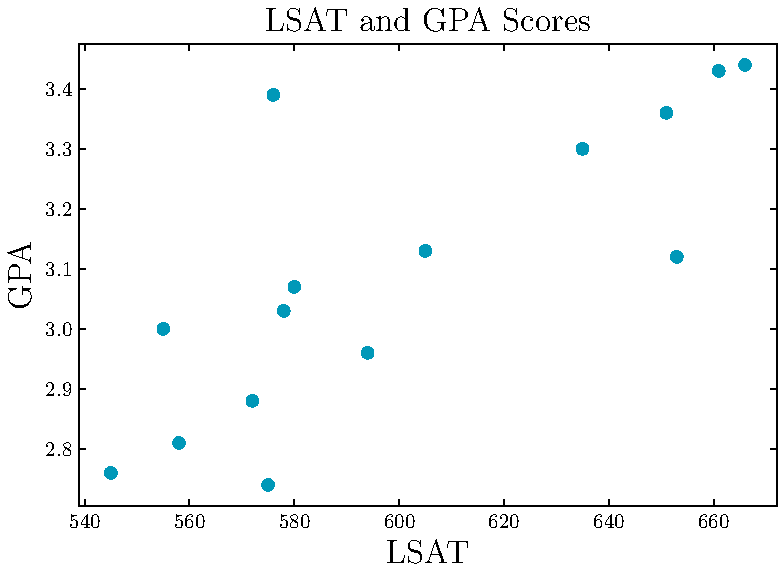
\includegraphics[width=1.0\textwidth]{chap8/chap8ex1i.eps}
\end{center}

And  calculate the plug-in estimate of the correlation as \(0.7764\). For \(B = 1000\) number of samples, we bootstrap the correlation, which has  standard error \(0.1387\). This gives us for the confidence intervals 

\renewcommand{\arraystretch}{2}
\begin{center}
\begin{tabular}{|c|c|}
	\hline
	Normal & \(\left( 0.5045, 1.0482 \right) \) \\
	\hline
	Pivotal & \(\left( 0.5944, 1.1100 \right) \) \\
	\hline
	Percentile & \(\left( 0.4428, 0.9583 \right) \) \\
	\hline
\end{tabular}
\end{center}

\begin{python}
est = pearsonr(LSAT, GPA)[0]

b = len(LSAT)
B = 1000

def bootstrap():
        bootstrapsamples = []
        for i in range(0,B):
            pairsample = choices(list(zip(LSAT,GPA)), k=b) 
            pairsample_unzip = list(zip(*pairsample))
            corrbootsample = pearsonr(pairsample_unzip[0], 
	    		     pairsample_unzip[1])[0]
            bootstrapsamples.append(corrbootsample)
        return bootstrapsamples;

sampleboot = bootstrap()

seboot = np.std(sampleboot)

normci = (est - 1.96*seboot, est + 1.96*seboot)
pivotalci = (2*est - np.quantile(sampleboot, 0.975), 
	     2*est - np.quantile(sampleboot, 0.025))
percentileci = (np.quantile(sampleboot, 0.025), 
		np.quantile(sampleboot, 0.975))
\end{python}

\begin{center}
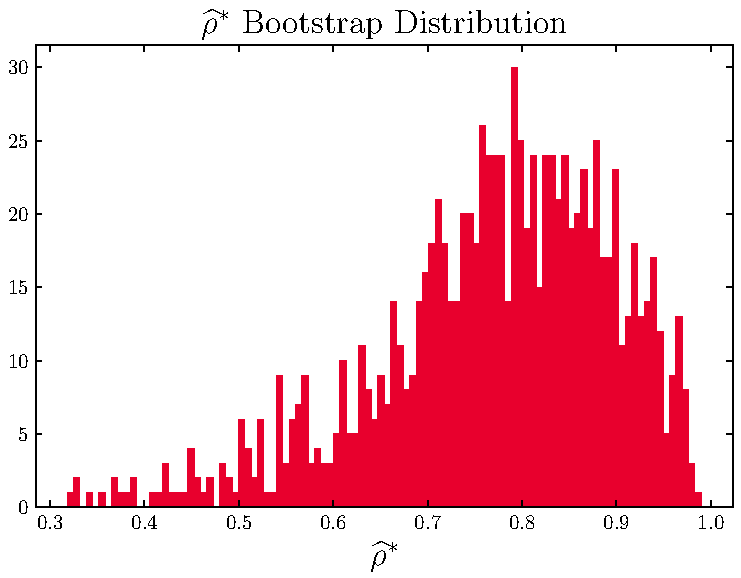
\includegraphics[width=1.0\textwidth]{chap8/chap8ex1ii.eps}
\end{center}

% QUESTION 2
\qs{8.6.2}{\textsf{(Computer Experiment.)} Conduct a simulation to compare the various bootstrap confidence interval methods. Let \(n = 50\) and let \(T \left( F \right) = \int \left( x - \mu  \right)^{3} \ dF \left( X \right) /\sigma^{3}\) be the skewness. Draw \(Y_{1}, \cdots, Y_{n} \sim N \left( 0,1 \right) \) and set \(X_{i} = e^{Y_{i}}, i = 1, \cdots, n\). Construct the three types of bootstrap 95 percent intervals for \(T \left( F \right) \) from the data \(X_{1}, \cdots, X_{n}\). Repeat this whole thing many times and estimate the true coverage of the three intervals.}

On visual inspection, the distribution of our exponentiated normal sample is extraordinarily skewed.

\begin{center}
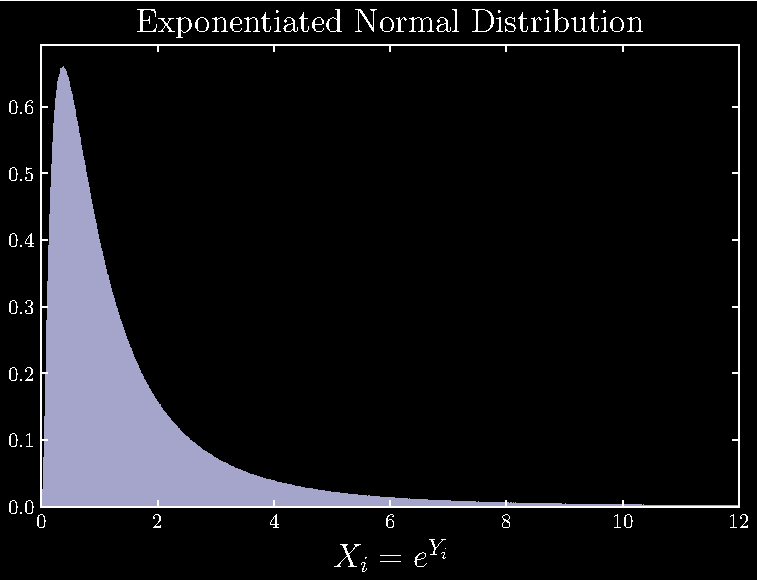
\includegraphics[width=1.0\textwidth]{chap8/chap8ex2expnormal.eps}
\end{center}

Empirically calculating the skew from a sample size of \(10^{8}\) produces values between \(6.1\) and \(6.2\). To bootstrap the skew over many iterations, as well as examining what ensues when we increase the size of the sample (from \(n = 50\)), we implement multiprocessing to conscript more CPUs to assist in the computation.

For each of the three confidence interval, we first repeat the sampling for the bootstraps \(N\) times, tabulate the standard error and construct the confidence interval, check if the true skew of distribution lies within the confidence interval, and calculate the coverage. In the second graph, we hold the number of repetitions at \(R = 100\), and instead calculate the coverage as it grows from \(N = 10\) to \(N = 1000\) samples. The relevant code is located in the chapter GitHub repo folder. 

\vspace{-3pt}
\begin{center}
\setlength{\lineskip}{-1pt}
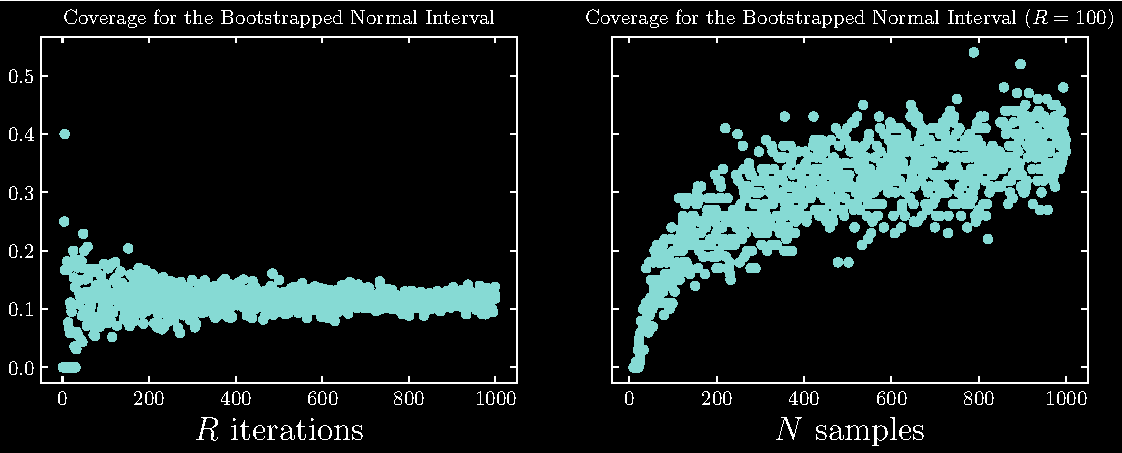
\includegraphics[width=1.0\textwidth]{chap8/chap8ex2normal.eps}
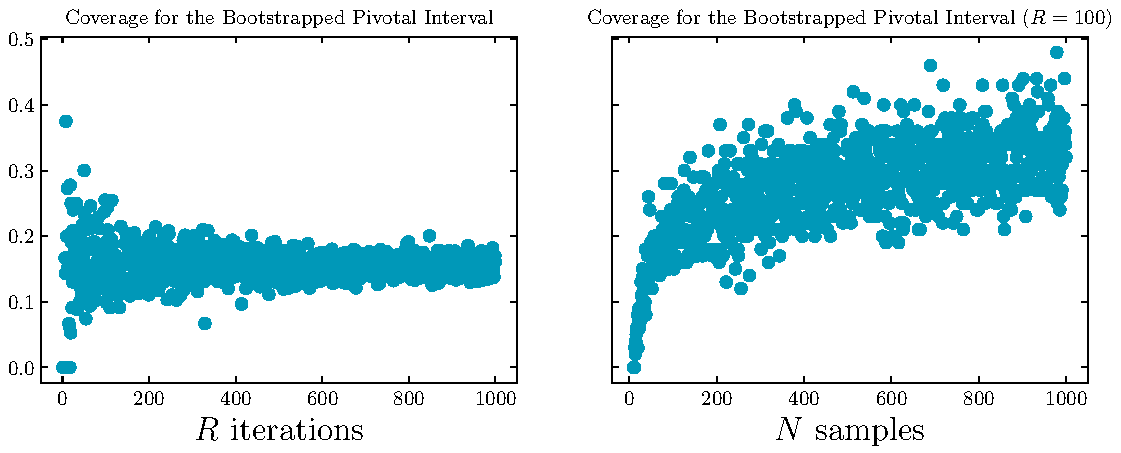
\includegraphics[width=1.0\textwidth]{chap8/chap8ex2pivotal.eps}
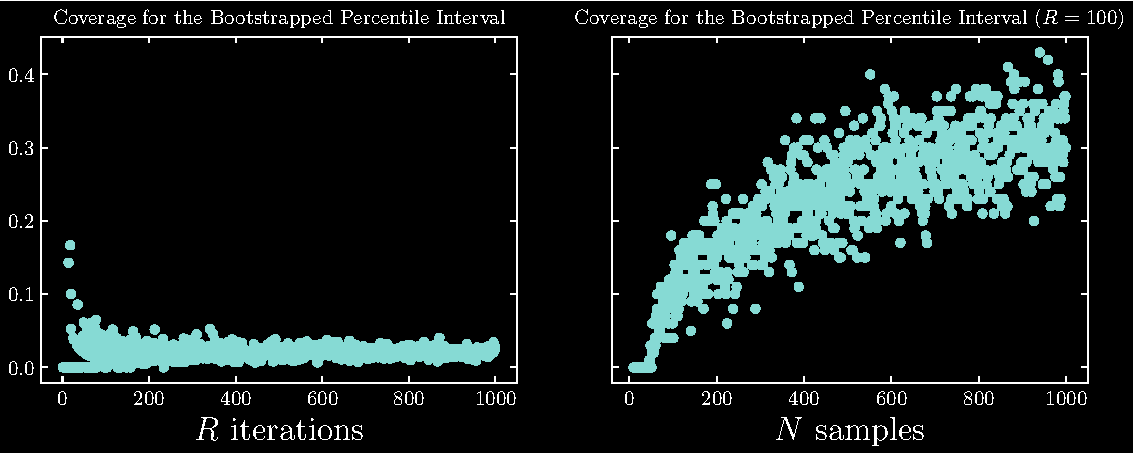
\includegraphics[width=1.0\textwidth]{chap8/chap8ex2percentile.eps}
\end{center}

% QUESTION 3
\qs{8.6.3}{Let
\[
	X_{1}, \cdots, X_{n} \sim t_{3}
\]
where \(n = 25\). Let \(\theta = T \left( F \right) = \left( q_{.75} - q_{.25} \right) / 1.34\) where \(q_{p}\) denotes the \(p^{th}\) quantile. Do a simulation to compare the coverage and length of the following confidence intervals for \(\theta\):

\begin{enumerate}[]
	\item Normal interval with standard error from the bootstrap,
	\item bootstrap percentile interval, and
	\item pivotal bootstrap interval.
\end{enumerate}}

\begin{center}
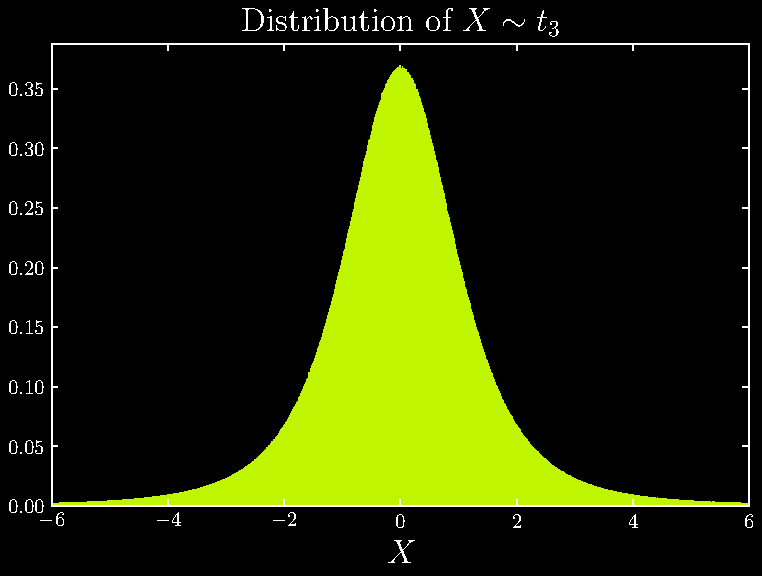
\includegraphics[width=1.0\textwidth]{chap8/chap8ex3tdistribution.eps}
\end{center}

\begin{center}
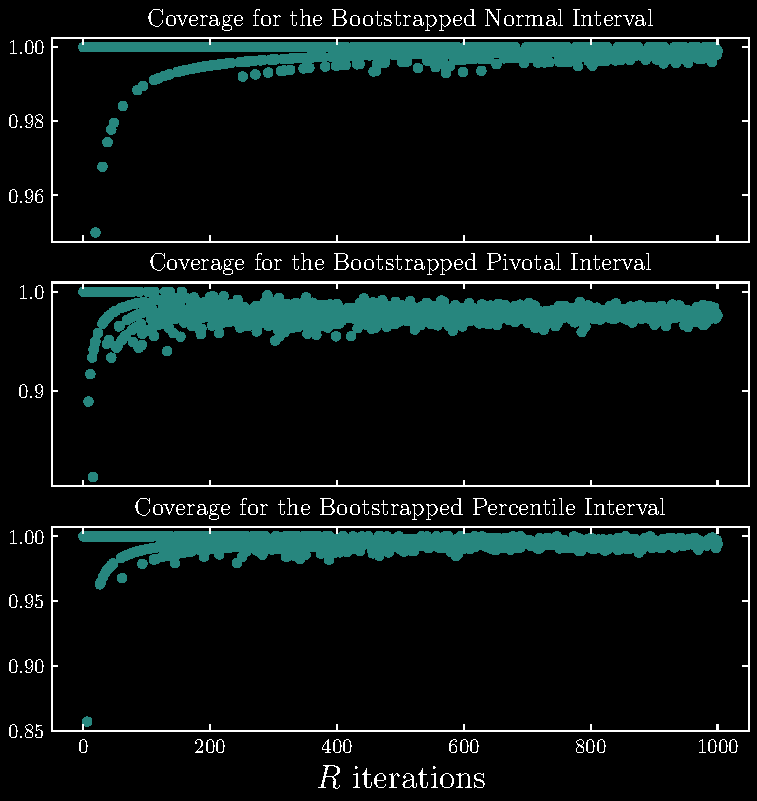
\includegraphics[width=1.0\textwidth]{chap8/chap8ex3.eps}
\end{center}

% QUESTION 4
\qs{8.6.4}{Let \(X_{1}, \dots, X_{n}\) be distinct observations (no ties). Show that there are
\[
	\binom{2n-1}{n}
\]
distinct bootstrap samples.

Hint: Imagine putting \(n\) balls into \(n\) buckets.}
\begin{proof}[Proof] 
First, let us establish some conceptual points to clarify the hint. Suppose we have three unique observations \(X_{1}, X_{2}, X_{3}\). Then we gather our bootstrap samples, obtained \textit{with} replacement. The set of all samples we can get is (using shorthand to denote that the first, second, and third digits in the sequence correspond to \(X^{*}_{1}, X^{*}_{2}, X^{*}_{3}\) equal to the first, second, or third observation):
\[
	\begin{tabular}{c c c}
		111 & 112 & 123 \\
		222 & 113 &  \\
		333 & 221 &  \\
		 & 223 &  \\
		 & 331 &  \\
		 & 332 &  \\
	\end{tabular}
\]
Now, consider 3 (identical) balls with 3 bins. One way we could place the balls in the bins is to put all of them in bin 1. Or two in bin 1, and one in bin 2. One in each bin is also an option. In other words, the combinatorial problem of how to place \(n\) balls in \(n\) bins is precisely the equivalent conundrum to resolve. The three bootstrap samples are the balls, and the specific choice of observation (\(X_{1}, X_{2}, X_{3}\)) are analogous to the choice of bin.

Developing the combinatorial theory to complete the proof is beyond the scope here.\footnote{See \textit{Combinatorics: Discrete Mathematics and its Applications}, Nicholas A. Loehr} In short, the number of ways to fit \(k\) identical balls into \(n\) bins labeled \(1, \dots, n\) is
\[
	\binom{k + n - 1}{k} = \frac{\left( k + n - 1 \right)!}{k! \left( n-1 \right)!}
\]
For \(k = n\) balls, we have
\[
	\binom{2n - 1}{n} = \frac{\left( 2n-1 \right)!}{n! \left( n-1 \right)!}
\]
\end{proof}

\end{document}
